%\documentclass[letterpaper]{article}
\documentclass{article}
\usepackage{hyperref}
\usepackage{natbib,alifeconf}
\newcommand\tab[1][1cm]{\hspace*{#1}}

\usepackage{xcolor}
\usepackage{amsmath}

\makeatletter
\def\mcolor#1#{\@mcolor{#1}}
\def\@mcolor#1#2#3{%
  \protect\leavevmode
  \begingroup
    \color#1{#2}#3%
  \endgroup
}
\makeatother

\newcommand{\annotate}[3]{
\mcolor{#1}{\overbrace{#3}^\text{#2}}
}

\newcommand{\plot}[3]{
    \begin{figure}[h]
        \includegraphics[keepaspectratio=true,scale=#3]{plots/#1}
        \caption{#2}
        \label{fig:#1}
    \end{figure}
}

\newcommand{\sitem}[1]
{
    \begin{itemize}
        \item #1
    \end{itemize}
}

\definecolor{orange}{HTML}{f7c767}
\definecolor{blue}{HTML}{67E6F7}
\definecolor{green}{HTML}{bdf767}
\definecolor{purple}{HTML}{f467f7}
\definecolor{red}{HTML}{fc4475}

\usepackage{tikz}
\usetikzlibrary{arrows.meta}

% \title{Models of Decision Making in the Rock Ant Temnothorax Albipennis}
\title{Feedback Loop based Decision Making for the Rock Ant Temnothorax Albipennis}
\date{\today}
\author{Lucas Saldyt}
\begin{document}
\maketitle

\begin{abstract}
    Rock ants (Temnothorax Albipennis) display the captivating ability to choose optimally between nest sites in a partially decentralized, error correcting, and self-organizing process.
    Often, Temnothorax nests are fragile, which leads to frequent colony migrations where there are multiple options for a new nest site.
    This paper reviews and simplifies models of Temnothorax nest-decision making, and reduces them to a simple feedback loop.
    Then, this paper shows the dynamics of the decision feedback loop, and how it relies, in particular, on the ability of individuals to make accurate independent assessments.
\end{abstract}

\section{Introduction}

%% Ants prefer thicker, darker nests [ Mallon 2001 ].

Ant nest choice is deeper than it may initially seem.
First, the entire colony needs to cooperate during migration, which is a potentially risky task.
In particular, because individual ants find new nests stochastically, there is potential for colony splitting when different ants select different nests (i.e. ant \emph{a} leads half of the colony to nest $1$, while ant \emph{b} leads the other half of the colony to nest $2$).
However, there exist natural mechanisms to prevent this.
Namely, the ants will wait until the number of ants at a target colony exceeds a threshold, known as the quorum threshold (which is very similar in principle to the threshold in a drift-diffusion model) [cite drift diffusion model].
Additionally, carrying of active ants will fix colony splits, if they occur, and reverse tandem runs are theorized to do the same [cite Pratt 2002]. 

The quorum threshold influences a more general and equally important principle, the principle of \emph{graded commitment}.
In nature, graded commitment has discrete levels based on different recruiting mechanisms: direct tandem runs (leading of other ants), transportations (carrying of other ants), and reverse tandem runs (leading of other ants, but in the opposite direction). 
Early work set out to describe the purpose and importance of each of these mechanisms, and this is discussed further along in the introduction.
Tandem runs represent a lower level of commitment than transportations, because tandem runs allow ants to learn the route, and then asses the new site for themselves, while transports do not allow route learning.
So, it is the quorum threshold which allows the transitions between these two levels of commitment, and the quorum threshold is reached by a feedback loop based on individual assessments of the site's quality. The final agent-based model with show an abstract version of these dynamics, where it is easier to see the importance of individual assessment.

\subsection{Summary (Mallon 2001)}

Temnothorax Albipennis colonies generally have relatively small sizes, which makes errors more likely. However, ants are able to use graded assessment to make decisions efficiently even though their colony size is small. In the agent based model, it is easy to see how unlucky noisy assessment can send the decision feedback loop in the wrong direction.

Additionally, a small number of comparisons are actually made between two nest sites.
Mallon 2001 publishes three experiments with $86\%, 46\%$ and $32\%$ direct comparison, which indicates the presence of decentralized behavior.
However, there is also good evidence that individual ants that have seen two sites know which is the better of the two.

With respect to quorum threshold, ants seem to use peer rate estimation to decide on the quality of a particular colony: instead of counting the number of ants at a colony, they estimate the total number from the frequency of ants (if many ants are seen over a brief period of time, then an ant knows that the current location has a large number of ants).


%% \begin{itemize}
%%     \item How does small colony size affect decision making?
%%         \sitem{\mcolor{red}{Graded assessment} affects the colony feedback loop}
%%     \item What proportion of comparison is by individuals as opposed to at the colony level? 
%%     \sitem{\mcolor{red}{$86\%, 46\%, 32\%$} for different colonies.}
%%     \sitem{Direct comparison is \mcolor{red}{not crucial} for choosing the optimal site and therefore the decision is \mcolor{red}{decentralized}}
%%     \item What physical observations act as cues for behavior? 
%%         \sitem{\mcolor{red}{Nestmate interaction rate} for estimation of colony/environment state}
%% \end{itemize}


\subsection{Summary (Pratt 2002, 2005)}

Each recruitment mechanism has different advantages. Tandem running allows learning of the route to a nest as well as the deposition of pheromones along the route. 
Later in the decision process, ants switch to ``transport`` recruitment, where they literally carry other ants. 
This mechanism triggers when ants know that a destination nest has a large number of ants (is above the quorum, or threshold, which is estimated by encounter rate), and as discussed previously, this threshold acts as error-correction.

Faster recruitment to better sites allows decentralized optimal choice without direct comparison.
In other words, when an ant encounters a good site, it recruits to that site very quickly, which causes positive feedback when subsequent ants encounter and recruit to the same site.
This can be seen in the population equations from Pratt 2002, where incoming ants depend on the number of recruiting ants.

%%        \begin{itemize}
%%            \item What is the purpose of multiple recruitment mechanisms? (Pratt 2002, 2005)
%%                \sitem{Tandem runs allow route learning and pheromone depositing}
%%                \sitem{\mcolor{red}{Graded commitment} allows error-correction and optimal decision making.}
%%                \sitem{Recruitment \mcolor{red}{accelerates} when transport begins ($3x$ speed)}
%%            \item How do individuals choose between recruitment mechanisms? (Pratt 2005)
%%                \sitem{Transports preffered once \mcolor{red}{quorum} is met}
%%            \item How does decentralization happen without direct comparison? (Pratt 2005)
%%                \sitem{Recruit to better sites faster $\rightarrow$ \mcolor{red}{positive feedback}}
%%        \end{itemize}

Reverse tandem runs had no single explaining mechanism, but it was hypothesized that they either stimulated transport by idle workers, or fixed nest-splitting that would be more common in nature than in the lab.
The quorum requirement seems to assist the ants in making optimal choices by acting as a general error correction mechanism --- it delays decision making in case ants have chosen a sub-optimal nest, and this decreases the likelihood of colony splitting.

\subsection{Summary (Granovskiy 2012)}

Granovskiy 2012 simplifies many of the ideas in the previous 2005 agent-based model.
It still has four macro-states: Exploring, Assessing, Canvassing (Leading), and Committed (Carrying).
However, it is simplified each of them so that they contain only the substates: search and at-nest, as well as their respective specialized actions (tandem runs for the canvassing population, and transport and reverse tandem runs for the committed populations). 
Also, assessing ants can begin recruiting once they accept a nest.

Additionally, there is the possibility that any searching ant can be picked up and carried to a nest nest, and any ant can be led by tandem run.
Otherwise, this model does not have any extra features from the 2005 model, but still seems to perform similarly.


%%       \begin{itemize}
%%               \sitem{Selection of an individual ant's ``home`` nest}
%%           \item How is quorum detected?
%%               \sitem{Ants likely use \mcolor{red}{rate estimation} rather than literal counting}
%%           \item \mcolor{red}{\em{Important parts of the decision process occur at the individual level}}
%%       \end{itemize}
%% \section{Previous models}
%% 
%%   \subsection{2002 Model Overview}
%%   S.Pratt 2002 contains an ODE model, which models a colony of $N$ ants, where proportion $p$ are active. \\
%%       $M$ sites (in practice $~2-12$ sites). \\
%%       Four population classes: 
%%       \begin{itemize}
%%           \item $S$: Searching (At destroyed nest or between nests) \mcolor{black}{(Initially $Np$)}
%%           \item $A_i$: Assessing a nest $i$ \mcolor{black}{(Initially 0)}
%%           \item $R_i$: Recruiting to a nest $i$ \mcolor{black}{(Initially 0)}
%%           \item $P_i$: The passive population at nest i \mcolor{black}{($P_0 = N(1-p), P_i = 0$)}
%%       \end{itemize}
%% 
%%   \subsection{Overview of Pratt 2002 Equations (Colors showing flow of ant population)}
%%       \Large
%%       \begin{equation}
%%       \begin{aligned}
%%           & \frac{ds}{dt} = - \sum_{j=1}^m \mcolor{black}{u_js} - \sum_{j=1}^m \mcolor{black}{\lambda_ji(r_j, s)} \\
%%           & \frac{da_i}{dt} = \mcolor{black}{u_is} + \mcolor{black}{\lambda_ji(r_j, s)} + \sum_{j \neq i}^m \mcolor{black}{(\rho_{ji}a_j - \rho_{ij}a_i)} - \mcolor{black}{k_ia_i} \\
%%           & \frac{dr_i}{dt} = \mcolor{black}{k_ia_i} + \sum_{j \neq i}^m \mcolor{black}{(\rho_{ji}r_j - \rho_{ij}r_i)} \\
%%           & \frac{dp_i}{dt} = \annotate{black}{causes overflow if unchecked}{\phi_ij(r_i, p_0)} - \annotate{black}{fix: subtract moved ants}{\phi_{dest}j(r_{dest},p_0)}
%%       \end{aligned}
%%       \end{equation}
%%   \subsection{Search population}
%%       \Large
%%       \begin{equation}
%%       \frac{dS}{dt} = - \sum_{j=1}^M \annotate{black}{Rate of finding nest $j$}{u_j}*S \\  
%%       - \sum_{j=1}^M \annotate{black}{Ants led by tandem run}{\lambda_jI(R_j, S)} 
%%       \end{equation}
%%   \subsection{Assessment population}
%%       \Large
%%       \begin{equation}
%%       \frac{dA_i}{dt} = \annotate{black}{Ants that find nest $i$ and begin assessing it}{u_iS} \\ 
%%       + \annotate{black}{Ants led by tandem run}{\lambda_jI(R_j, S)} \\
%%       + \sum_{j \neq i}^M \annotate{black}{Ants encountering alternative sites}{(\rho_{ji}A_j - \rho_{ij}A_i)} \\ 
%%       - \annotate{black}{Ants that become recruiters}{k_iA_i} \\
%%       \end{equation}
%%   \subsection{Recruitment population}
%%       \Large
%%       \begin{equation}
%%           \frac{dR_i}{dt} = \annotate{black}{Ants that become recruiters}{k_iA_i} \\
%%           + \sum_{j \neq i}^M \annotate{black}{Ants encountering alternative sites}{(\rho_{ji}R_j - \rho_{ij}R_i)}
%%       \end{equation}
%%   \subsection{Passive population}
%%       \Large
%%       \begin{equation}
%%           \frac{dP_i}{dt} = \underbrace{\annotate{black}{Per capita transport rate}{\phi_i} * \annotate{black}{Quorum requirement}{J(R_i, P_0)}}_\text{Carried passive ants}
%%       \end{equation}
%%   \subsection{Auxilary Functions}
%%       \Large
%%       Tandem/Carrying switching rule:
%%       \begin{equation}
%%           I(R_i, S) = 
%%           \begin{cases}
%%               & R_i,  \text{ if } \annotate{black}{Recruiters below threshold}{R_i < T} \\
%%               &       \text{     and } \annotate{black}{While there are recruitable ants}{S > 0}\\
%%               & 0, \text{ otherwise}
%%           \end{cases}
%%       \end{equation}
%% 
%%   \subsection{Auxilary Functions}
%%       \Large
%%       Quorum rule:
%%       \begin{equation}
%%           J(R_i, P_0) = 
%%           \begin{cases}
%%               & 0,  \text{ if } \annotate{black}{Recruiters below threshold}{R_i < T} \\  
%%               &     \text{     or } \annotate{black}{Edge case: migration has finished}{P_0 = 0}\\
%%               & R_i, \text{ otherwise}
%%           \end{cases}
%%       \end{equation}
%% 
%%   \subsection{Assumptions}
%%       \begin{itemize}
%%           \item Ants always move exclusively out of the searching state
%%           \item Finding/Recruitment/Switching/Conversion rates are all constant per nest
%%           \item Requires detailed parameter estimation
%%       \end{itemize}
%% 
%%   \subsection{Diagram of ODE model (Pratt 2002)}
%% 
%%   \subsection{The agent based model (Pratt 2005)}
%% 
%%   \subsection{Important differences between the models (In order of subjective importance)}
%%       \begin{itemize}
%%           \item Ants remember their ``home`` nest.
%%           \item Commitment level is separated from individual actions 
%%               \sitem{(i.e. an ant can follow even in the committed state)}
%%               \sitem{Also allows for further parameterization}
%%           \item Intentionally makes the model more brittle so that it can be further tested empirically. 
%%               \sitem{A general model is potentially harder to disprove}
%%           \item Adds a simple ``at-nest`` action 
%%           \item Minute differences (potential for ants to get lost)
%%       \end{itemize}
%% 
  \section{Proposed Ordinary Differential Equation Model}

  The proposed model begins with an improved set of ordinary differential equations, based on Pratt 2002.
  It contains equations for five separate populations: 
  \begin{itemize}
      \item $S$, the searching population (not at any nest)
      \item $A_i$, the assessing population at nest $i$
      \item $L_i$, the leading (forward-tandem-running) population at nest $i$
      \item $C_i$, the carrying (transport) population at nest $i$
      \item $P_i$, the passive population at nest $i$. 
  \end{itemize}
  The model focuses on the following:
  \begin{itemize}
      \item Splitting the $R_i$ population from S. Pratt 2002 into the $L_i$ and $C_i$ populations.
      \item Replacing the two switching equations $I()$ and $J()$ with dynamics switching between $L_i$ and $C_i$ based on a single switching equation $Q()$.
      \item Fixing unchecked growth in the original $P_i$ equations.
      \item Allowing transport of various passive populations, which will allow a split passive population to be fixed.
      %% \item Replacing switching in $A_i$ and $R_i$ with transitions to searching population. This reflects updates in S.Pratt 2005 and Granovskiy 2012 agent-based models.
      \item Adding transportation of the active searching population (but not the assessing, leading, or carrying populations).
  \end{itemize}

  Given $N$ ants, where proportion $p$ are active, the initial states are the following:
  \begin{itemize}
      \item $S = pN$
      \item $P_0 = (1-p)N$ 
      \item $A_i, L_i, C_i, P_i = 0$ 
  \end{itemize}

  The original model used the following parameters:\\

\begin{tabular}{ l | r }
    \hline
  $\mu_i$     & Likelihood of finding nest $i$\\
  $\lambda_i$ & Proportion led by leaders to $i$\\
  $\rho_{ij}$ & Switching rates between nests $i$ and $j$\\
  $k_i$       & Acceptance probability for nest $i$\\
  $\phi_i$    & Rate for carrying passive ants to nest $i$\\
    \hline
\end{tabular} \\

The updated model builds on this list, but renames old parameters to make them more intuitive. Estimated values are from (Pratt 2002): \\

\begin{tabular}{ l | c | c | r }
    \hline
  Name          & 2002        & Value & Description (units = rate)\\ \hline
  {$\phi_i$}      & $\mu_i$     & 0.13 & Finding nest $i$\\
  {$\lambda_i$}   & $\lambda_i$ & 0.033 & Led by leaders to $i$\\
  {$\alpha_i$}    & $k_i$       & 0.015, 0.02 & Assessors who accept nest $i$\\ \hline
  {$\tau$}        & $\phi_i$    & 0.001  & Uniform transport rate $i$\\
  %% {$\sigma_{Ai}$} & \em{New}    & 0.0195 & Assessing ants enter search from $i$\\
  %% {$\sigma_{Li}$} & \em{New}    & 0.018  & Leading ants enter search from $i$\\
  %% {$\sigma_{Ci}$} & \em{New}    & 0.0044 & Carrying ants enter search from $i$\\
  \hline
\end{tabular} \\

\subsection{Parameter Descriptions} 

$\phi_i$, previously $\mu_i$, describes the rate at which search ants find nest $i$. 
Generally, this will be used to describe nests that are at different distances from the original destroyed nest. \\
$\lambda_i$ describes the rate at which ants are led by leaders to nest $i$. 
Differences in $\lambda_i$ would describe nests which were led to faster. \\
$T$ is simply the quorum threshold, and is a free variable meant to be experimented with.
Pratt 2002 found that a value between $8$ and $30$ was best. \\
$\alpha_i$, previously $k_i$, describes the rate at which assessors accept a nest and begin recruiting.
It is this parameter which allows a rapid positive feedback loop to occur, and this is largely responsible for optimal nest choice. \\
$\tau_{Pi}$, previously $\phi_i$ is the rate at which passive ants are transported to nest $i$.
However, this model introduces a few new parameters, based on the agent based models in [TODO: Gravinvosky?] and Pratt 2005. 
For instance, $\tau_{Si}$ describes the transport of searching ants. 
TODO: Should there also be transport of other active ants? \\
%% $\sigma$ describes the rate at which ants in an active state ($A_i$, $L_i$, or $C_i$) enter searching again.
%% For instance, $\sigma_{Ai}$ would denote the rate at which assessing ants enter search from nest $i$.

\subsection{Proposed Equations and Descriptions}

\subsubsection{Searching population equation}
\hfill\\

The following equation describes the searching population, which starts as $Np$.
\begin{equation}
      \frac{dS}{dt} = S * \sum_i \big[- \phi_i - \lambda_iL_i - \tau C_i 
          %% + \sigma_{Ai}A_i + \sigma_{Li}L_i + \sigma_{Ci}C_i 
      \big]
\end{equation}

The first term, $\phi_i$, describes ants that encounter new sites and enter the assessment population.
$\lambda_iL_i$ describes ants being led to new sites and becoming assessors. $L_i$ is included here because the presence of more leading ants will increase the rate at which ants are led to new sites (i.e. ten leading ants lead ants faster than a single ant). Therefore $\lambda_i$ is proportional to $L_i$.
$\tau C_i$ describes ants that are transported to new sites. As with the previous term, $\tau$ is a rate per individual in $C_i$.
%% Lastly, the $\sigma$ terms describe ants that exit other active states and begin searching, each with an independent rate.

\subsubsection{Assessing population equation}
\hfill\\

The following equation describes the assessment populations, which start at $0$:
%% \begin{equation}
\begin{multline}
    \frac{dA_i}{dt} = S * [\phi_i + \lambda_iL_i - \alpha_iA_i] \\
    + \tau \sum_{j \neq i, j} \big[ C_i * {(S + L_j + C_j + A_j)} - C_j * {A_i} \big] \\ %%- \sigma_{Ai}A_i] 
\end{multline}
%% \end{equation}

The first three terms match the first three terms of the search-population equation.
$\phi_iS$ describes incoming ants that have found the nest themselves, $\lambda_iL_iS$ describes ants that were led to the nest $i$, and $\alpha_iA_i$ describes ants that accept a nest and begin recruiting.
Lastly, $$\tau \sum_{j \neq i, j} \big[ C_i * {(S + L_j + C_j + A_j)} - C_j * {A_i} \big] \\ %%- \sigma_{Ai}A_i] 
$$ describes ants that were carried to $i$ from other populations, or were carried away to nest $j$. \\

%%$\sigma_{Ai}A_i$ describes ants that begin searching after assessing a nest, and lastly 

\subsubsection{Leading population equation}
\hfill\\

The following equation describes the leading populations, which starts at $0$.

\begin{equation}
        \frac{dL_i}{dt} = \alpha_iA_i - Q(i)L_i - \sum_{j \neq i, j} \tau C_jL_i %%-\sigma_{Ci}C_i \\
\end{equation}

First, the function $Q()$, defined below, returns $1$ if the nest $i$ is above the quorum threshold and $0$ otherwise. Therefore $1 - Q(i)$ is $0$ when the nest is above the quorum threshold and $1$ otherwise.
So, when the nest $i$ is above the quorum threshold, only the terms $-Q(i)L_i$ and $\sigma_{Li}L_i$ are active. $Q(i)L_i$ represents a movement of ants from leading to carrying. $\sigma_{Li}L_i$ represents leading ants deciding to enter the search state.
When the nest is below the quorum threshold, the first and third term are both active. $1-Q(i)\alpha_iA_i$ describes assessing ants entering the leading populations after accepting a nest, and $1-Q(i)Ci$ describes (potentially) carrying ants reverting to the leading state.

\subsubsection{Carrying population equation}
\hfill\\

The following equation describes the carrying populations, which starts at $0$:

\begin{equation}
        \frac{dC_i}{dt} = Q(i)L_i - \sum_{j \neq i, j} \tau C_jC_i %% - \sigma_{Ci}C_i \\
\end{equation}

Similarly to the leading population equations, $Q()$ acts as a switch. When the nest $i$ is above the quorum threshold, assessing ants will enter the carrying population directly through the $Q(i)\alpha_iA_i$ term and leading ants are converted through the $Q(i)L_i$ term.
The term $(1-Q(i))C_i$ describes ants that (potentially) revert to the leading state. 
%% Lastly, the term $\sigma{Ci}C_i$ describes ants that enter the searching state from carrying.

\subsubsection{Passive population equation}
\hfill\\

The following equation describes the passive population dynamics. Initially, $P_0 = (1-p)N$ and otherwise $P_i = 0$:
\begin{equation}
\begin{aligned}
        \frac{dP_i}{dt} = \sum_{j \neq i} [\tau P_j C_i - \tau P_i C_j] \\
\end{aligned}
\end{equation}

Essentially, the first term $\tau P_jC_i$ desribes ants being moved to site $i$ from site $j$, while the second term describes ants being moved from site $i$ to site $j$.

\subsubsection{Quorum function}
\hfill\\

The $Q()$ switching function is defined as follows, and should be self explanatory. Potentially, (TODO) $P_i$ population should not be counted (but in simulation, this is not a contributing factor):

\begin{equation}
\begin{aligned}
  & Q(i) = 0, \text{if    } \sum [A_i + L_i + C_i + P_i] \leq T \\
  & Q(i) = 1, \text{otherwise} \\
\end{aligned}
\end{equation}

These equations do not account for reverse tandem runs, but could be modified easily to do so (especially once tandem runs are better understood).



\section{Agent based model}

The analysis of the above models led to the creation of a very simple agent-based feedback loop model.
In essence, individual ants can make very accurate assessments of individual nests, and then recruit more quickly, based on the strength of this assessment.
This process creates a feedback loop, where better nests are assessed by more ants at a higher rate.
The purpose of this model is not to replicate all of the events that occur in nature (such as the inividual tandem running or carrying actions), but instead to model the core dynamics of general distributed choice performed by intelligent agents.

\subsection{Specific Implementation}
Consider a model with $N$ agents choosing between $M$ items.
Each agent has two properties:
\begin{enumerate}
    \item A \emph{commitment} strength, which is a floating point number that is initially zero
    \item A \emph{source} item, which is an integer representing the item that an individual agent considers optimal.
\end{enumerate}
Each agent has two actions:
\begin{enumerate}
    \item Recruitment to \emph{source} item, triggered with probability $c$, which is the \emph{commitment} strength of the agent.
    \item Discovery of new items, triggered first with probability $1 - c$. Then a random (possibly weighted) item (or no item at all) is chosen to be encountered. Once a new item is found, \emph{commitment} strength is updated if and only if the item is superior.
\end{enumerate}

For instance, consider a simple scenario with two items that are both found at probability $0.013$ per timestep, and have qualities of $0.02$ and $0.015$ respectively.
Since agents start with no commitment strength, agents will trigger the discovery action.
Once the discovery action is triggered, a multinomial choice is made, with the following chances:
\begin{itemize}
    \item $0.013$ chance of finding item $1$.
    \item $0.013$ chance of finding item $2$.
    \item $0.974 = 1 - 2 * 0.013$ chance of doing nothing.
\end{itemize}

Suppose an agent encounters item $1$. This agent's commitment strength is now updated to $0.02$, and this agent now recruits to nest $1$ with this probability.
While simple, this model is able to explain the important behavior in Temnothorax decision making.

\section{Results}

Each of the above models was tested independently. Code is available \href{https://github.com/LSaldyt/temnothorax}{online} \footnote{https://github.com/LSaldyt/temnothorax} so that results can be replicated. 

\subsection{ODE Results}
Originally, Pratt (2002) investigated quorum threshold ($T$), but their model depends largely on two other parameters: $\alpha$, for nest quality, and $\phi$, for nest distance.
Convergence time was explored as a function of these three parameters. 
Convergence time is defined as the number of timesteps taken to reach a population of $95\%$ at the correct nest.
A cutoff of $1000$ iterations was used, such that a simulation running for longer than this was considered divergent (this is similar to how the mandelbrot set is calculated).

Figure \ref{fig:convergence_times} explores convergence as a function of quorum threshold and quality of first nest. 
$\beta$ (quality of second nest) is kept at $0.05$ while $\alpha$ (quality of first nest) is varied.
At the same time, quorum threshold is also varied from $0$ to $30$ in increments of $2$.
This results in high convergence times centered around equal nest qualities, which shows the intuitive result that nests of similar qualities are hard to pick between.
Additionally, a lower quorum threshold actually \emph{increases} convergence time, which is a counter-intuitive result.

\plot{convergence_times}{Convergence times based on nest quality}{0.6}

Figure \ref{fig:distance_convergence_times} explores convergence as a function of quorum threshold and distance of second nest. 
$\phi_a$ (distance of first nest) is kept at $0.01$ while $\phi_b$ (distance of second nest) is varied.
At the same time, quorum threshold is also varied from $0$ to $30$ in increments of $2$.

In Figure \ref{fig:distance_convergence_times}, for $T > 10$, there is a clear pattern between threshold and nest distance. 
For uniform (i.e. equal) nest distances, increasing quorum threshold increases convergence time.

In Figure \ref{fig:distance_convergence_times_low_T}, for $T <= 10$\dots

\plot{distance_convergence_times}{Convergence times based on nest distance}{0.6}

\plot{distance_convergence_times_low_T}{$T < 10$ convergence times}{0.6}

\plot{agent_based_population_model}{Basic population model}{0.6}

% 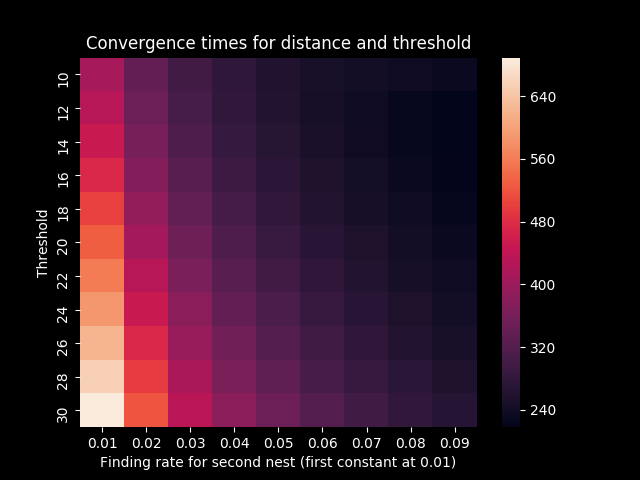
\includegraphics[scale=1.0]{distance_convergence_times_t_over_10}
% 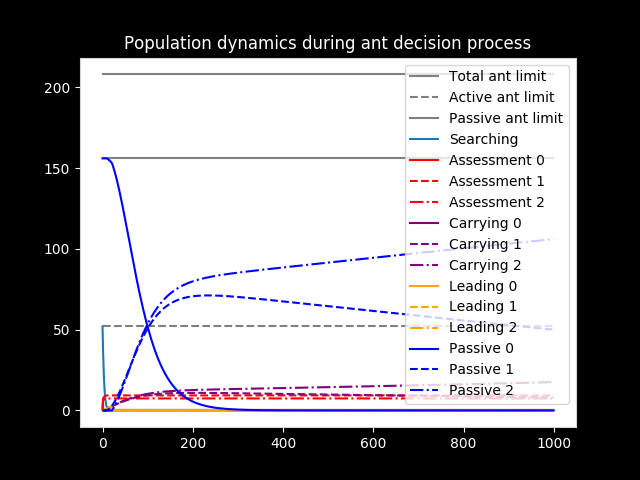
\includegraphics[scale=1.0]{populations}
% agent_based_population_model.png  convergance_times.png  distance_convergance_times_low_T.png  distance_convergance_times.png  distance_convergance_times_t_over_10.png  populations.png


\subsection{Bibliography}
  \bibliography{sources/insects,sources/brains,sources/ant_system,sources/networks,sources/misc}

\footnotesize
\bibliographystyle{apalike}
\bibliography{sample}


\end{document}
